\documentclass[runningheads]{llncs}
\usepackage{hyperref}

\usepackage{amsmath, amssymb}
% For moving the title up
\usepackage{titling}
\usepackage{mystyles}
\usepackage{mymacros}

\usepackage{float}
\usepackage{caption}
\usepackage{chngcntr}
\usepackage{tikz}
\usepackage{stmaryrd}

\captionsetup{labelfont=bf, justification=raggedright, singlelinecheck=false}
\counterwithin{figure}{section}
\DeclareCaptionType[fileext=los,placement=H]{protocol}
\counterwithin{protocol}{section}
\DeclareCaptionType[fileext=los,placement=H]{functionality}
\counterwithin{functionality}{section}

\newenvironment{afigure}[2]
    {
    \begin{figure}[H]
    \begin{mdframed}[align=left]
    \caption{\label{#1} \textbf{#2}}
    }
    {
    \end{mdframed}
    \end{figure}
    }

\newenvironment{aprotocol}[2]
    {
    \begin{protocol}
    \begin{mdframed}[align=left]
    \caption{\label{#1} \textbf{#2}}
    }
    {
    \end{mdframed}
    \end{protocol}
    }

\newenvironment{afunctionality}[2]
    {
    \begin{functionality}
    \begin{mdframed}[align=left]
    \caption{\label{#1} \textbf{#2}}
    }
    {
    \end{mdframed}
    \end{functionality}
    }


\title{MPC for Group Reconstruction Circuits}

\begin{document}

\maketitle

\begin{abstract}
    \noindent In this work, we generalize threshold Schnorr signatures,
    {ElGamal encryption}, and a wide variety of other functionalities,
    using a novel formalism of \emph{group reconstruction circuits} (GRC)s.
    We construct a UC secure MPC protocol for computing these circuits
    on secret shared inputs, even in the presence of malicious parties.
    Applied to concrete circuits,
    our protocol yields threshold signature and encryption schemes
    with similar round complexity and concrete efficiency to
    functionality-specific protocols.
    Our formalism also generalizes to other functionalities,
    such as polynomial commitments and openings.
\end{abstract}

\section{Introduction}

Using threshold Cryptography~\cite{desmedt_society_1988,desmedt_threshold_1990},
a consortium of parties can split
a secret amongst themselves, such that no individual knows that
secret, and yet a sufficiently large quorum can
perform tasks using that secret, such as signing
or decrypting a message.

Particularly efficient protocols for threshold signing,
using Schnorr signatures~\cite{schnorr_efficient_1990},
have been devised
\cite{komlo_frost_2020,nick_musig2_2021,lindell_simple_2022}.
Similarly, efficient protocols for threshold
encryption can be constructed~\cite{desmedt_threshold_1990,shoup_securing_2001},
using ElGamal encryption \cite{elgamal_public_1985}.

These protocols are so efficient in large part due to the structure
of the underlying schemes being lifted to the threshold setting.
In particular, these schemes share the interesting property
that their computation is \emph{homomorphic} with respect
to their secret inputs.

To illustrate this, consider the computation of a Schnorr signature:
$$
\begin{aligned}
\textcolor{red}{k} &\xleftarrow{R} \mathbb{F}_q\\
K &\gets \textcolor{red}{k} \cdot G\\
e &\gets H(K, m)\\
s &\gets \textcolor{red}{k} + e \textcolor{red}{x}\\
(K&, S)
\end{aligned}
$$
Here, the secret values have been marked in red.
Notice that each value we compute is linear with respect
to the secrets it uses.
For example, if $\textcolor{red}{k} = k_0 + k_1$,
then we have $K = k_0 \cdot G + k_1 \cdot G$.
Similarly, if $\textcolor{red}{x} = x_0 + x_1$, then
we have $s = (k_0 + e x_0) + (k_1 + e x_1)$.
This property leads to very efficient protocols when the
secrets are shared linearly:
each participant can individually compute their portion of the result,
and then reconstruct the output together, by revealing
their portions and adding them together.
This computation needs to be done in stages, because the
homomorphic property is sometimes broken.
For example, the use of the hash function $H$ in this
scheme requires the parties to reconstruct $K$ before proceeding
with the rest of the computation.

This linear sharing of inputs is directly amenable to the threshold
setting.
This is because
the most common method of threshold secret sharing,
using polynomial interpolation~\cite{shamir1979share},
allows for a quorum of parties to locally convert their shares
into a linear sharing $x_1 + \ldots + x_n$ of the secret.

This homomorphic property is not unique to Schnorr signatures
and ElGamal encryption.
In fact, this property is present among a wide variety
of functionalities, including distributed key generation,
as well as polynomial commitments and openings~\cite{kate_constant-size_2010}.

In this work, we generalize these disparate functionalities,
and unify them under the novel framework of
\emph{group reconstruction circuits} (GRC).
These can be seen as a special class of programs which precisely
capture this property of staged homomorphic computation,
which is what makes threshold Schnorr signatures and
ElGamal encryption so efficient.

We then provide an efficient multi-party computation (MPC) protocol
for computing GRCs on linearly shared inputs.
In fact, our protocol provides MPC with \emph{commitment},
in the sense that it also verifies that the inputs
used correspond to publicly known commitments.
We prove that our protocol is secure under concurrent composition,
even in the presence of malicious participants,
within the UC framework \cite{canetti2001universally}.
This proof is done in the hybrid model,
using ideal functionalites for authenticated broadcast,
and for turning sigma protocols into non-interactive zero-knowledge
proofs of knowledge.
We also make use of a group $\mathbb{G}$ in which the discrete
logarithm is presumed to be hard.

The essence of our protocol is quite simple.
The computation
is separated into a series of rounds.
In each round, the parties locally compute their share
of the output for this round, which they then send
to the other participants.
The output is then reconstructed by adding all of these
shares together.
To prevent parties from cheating, we also require
that they prove, in zero-knowledge, that they correctly computed their output using inputs
which match their public commitments.
Because this computation is homomorphic,
there exists an efficient sigma protocol for
these proofs \cite{maurer_unifying_2009}.

Finally, we provide examples of GRCs for distributed key generation,
Schnorr signatures, ElGamal encryption, as well as polynomial commitments
and openings, which then automatically yield corresponding
protocols for threshold signatures, encryption, polynomial commitments,
etc.
The round complexity of these protocols are comparable
to their functionality-specific equivalents: we can do threshold
Schnorr signatures in 3 rounds, matching Lindell's scheme \cite{lindell_simple_2022},
and threshold ElGamal in a single round, which is optimal.

\section{Background}
\label{sec:background}

Throughout this paper, we let $\G$ denote a group of prime order $q$,
with generators $G$ and $H$. Let $\Fq$ denote the scalar field associated
with this group, and let $\Zq$ denote the additive group of elements
in this field. We also define $[n] := [1, \ldots, n]$.

By $\shared{x}$, we denote a linear secret sharing of some group element
$x$. This is a set $\{x_1, \ldots, x_n\}$ such that $\sum_i x_i = x$.

We make heavy use of group homomorphisms throughout this paper.
We let
$$
\varphi(P_1, \ldots, P_m) : \mathbb{A} \to \mathbb{B}
$$
denote a homomorphism from $\mathbb{A}$ to $\mathbb{B}$, parameterized
by some public values $P_1, \ldots, P_m$. Commonly $\mathbb{A}$
will be a product of several groups $\mathbb{G}_1, \ldots, \mathbb{G}_n$,
in which case we'd write:
$$
\varphi(P_1, \ldots, P_m)(x_1, \ldots, x_n)
$$
to denote the application of $\varphi$ to an element $(x_1, \ldots, x_n)$
of the product group. The public values $P_i$ are often left implicit.

We often write products $(x_1, \ldots, x_n)$ as a single vector
$\bx \in \mathbb{A}^n$. Operations between these vectors
are done element-wise, so we write $\bx + \by$ for ${(x_1 + y_1, \ldots, x_n + y_n)}$,
as well as $\bx \cdot G$ for $(x_1 \cdot G, \ldots, x_n \cdot G)$.

\subsection{Pedersen Commitments}

Pedersen commitments \cite{pedersen_non-interactive_1992}
are a key component of our protocol.
In their basic form, they allow one to commit to a value $x \in \Zq$. This
is done by sampling a random $\alpha \xleftarrow{R} \Zq$, and forming the commitment:
$$
\text{Com}(x, \alpha) := x \cdot G + \alpha \cdot H
$$
where $H$ is a generator of $\mathbb{G}$, independent from $G$.

This scheme is \emph{perfectly} hiding, because $\alpha \cdot H$ is
a random element of $\mathbb{G}$, completely masking $x \cdot G$.

On the other hand, this scheme is only \emph{computationally} binding. This
is because the discrete logarithm $H$ with respect to $G$ must be kept hidden.
If the discrete logarithm of $H$ is known, then it becomes possible to
\emph{equivocate}, by finding two different inputs $(x, \alpha)$ and $(x', \alpha')$
with the same commitment.

In fact, we can characterize this property more precisely: knowing
the discrete logarithm of $H$ is \emph{necessary} in order to be able
to equivocate.

\begin{lemma}
    \label{lemma:ped_dlog}
    Given two inputs $(x, \alpha) \neq (x', \alpha')$ such that ${\text{Com}(x, \alpha) = \text{Com}(x', \alpha')}$,
    it's possible to efficiently compute the discrete logarithm of $H$.
\end{lemma}

The proof is just a matter of algebra:

$$
\begin{aligned}
x \cdot G + \alpha \cdot H &= x' \cdot G + \alpha' \cdot H\\
(x - x') \cdot G &= (\alpha' - \alpha) \cdot H\\
\frac{(x - x')}{(\alpha' - \alpha)} \cdot G &= H\\
\end{aligned}
$$

Thus $(x - x') / (\alpha' - \alpha)$ is our discrete logarithm.

$\qed$

\subsubsection{Vector Pedersen Commitments}

It's useful to generalize this scheme to the case of a vector of scalars
${\textbf{x} \in \Zq^n}$. The randomness becomes a vector of the same
size, sampled as ${\balpha \xleftarrow{R} \Zq^n}$. We then define
an analogous commitment scheme by using scalar multiplication element-wise:
$$
\text{Com}(\bx, \balpha) := \bx \cdot G + \balpha \cdot H
$$
This generalization is naturally also perfectly hiding, and satisfies
an analogous property with regards to equivocation:

\begin{lemma}
    \label{lemma:ped_vec_dlog}
    Given two inputs $(\bx, \balpha) \neq (\bx', \balpha')$ such that
    $\text{Com}(\bx, \balpha) = \text{Com}(\bx', \balpha')$, it's possible
    to efficiently compute the discrete logarithm of $H$.
\end{lemma}

Since the two inputs are different, there exists an index $i$
such that $\bx_i \neq \bx_i'$ or $\balpha_i \neq \balpha_i'$.
From here we apply Lemma \ref{lemma:ped_dlog} with $(\bx_i, \balpha_i)$ and
$(\bx_i', \balpha'_i)$.

$\qed$

\subsubsection{On the Trusted Setup}

In theory, Pedersen commitments require a trusted setup, to generate
the group elements $G, H \in \mathbb{G}$.
We argue that this trusted setup isn't a concern in practice.
This is because the generator $G$
is usually part of the specification for the group being used,
and because there exist
efficient methods for hashing into elliptic curves \cite{icart_how_2009}.
This reduces the problem of generating $H$ to that of finding a credibly
``unbiased'' choice of seed to hash. This can be done in many ways.

One method would be to hash a canonical representation of $G$ as bytes in order
to produce $H$. Presumably, the generator $G$ was not chosen in such
a way as to produce an $H$ with a known discrete logarithm using
that specific method of hashing into the group.

Another method would be to use a public source of randomness,
such as public newspapers, lotteries
\cite{baigneres_trap_2015}, or Cryptographic protocols
designed to provide such a service \cite{fischer_public_2011}.

Now, while we can avoid a trusted setup with these methods in practice,
our security proof makes use of this setup.
Essentially, we'll prove that the security of our protocol reduces
to the hardness of the discrete logarithm problem in $\mathbb{G}$,
and to do this we need to be able to use an instance of the problem
as a setup for the participants in our simulation.

\subsection{Maurer's \texorpdfstring{$\varphi$}{varphi}-Proof}
\label{sec:maurer}

In \cite{maurer_unifying_2009}, Maurer generalized Schnorr's sigma 
protocol for knowledge of the discrete logarithm \cite{schnorr_efficient_1990} to a much larger class
of relations. In particular, Maurer provided a sigma protocol for
proving knowledge of the pre-image of a group homomorphism $\varphi$.
We denote this protocol as a ``$\varphi$-proof'', and recapitulate the scheme
here.

Given a homomorphism $\varphi : \mathbb{A} \to \mathbb{B}$, and a public value
$X \in \mathbb{B}$, a prover can demonstrate knowledge of a private
value $x \in \mathbb{A}$ such that $\varphi(x) = X$. The prover
does this by means of Protocol \ref{prot:phiproof}:

\begin{aprotocol}{prot:phiproof}{$\varphi$-Proof}
\[
\begin{aligned}
    &\textbf{Prover}&&\textbf{Verifier}\\
    &\text{knows } x \in \mathbb{A}&&\text{public } X \in \mathbb{B}\\
    \\
    &k \xleftarrow{R} \mathbb{A}&\\
    &K \gets \varphi(k)&\\
    &&\quad\overset{K}{\longrightarrow}\quad\\
    &&&c \xleftarrow{R} \mathbb{Z}/(p)\\
    &&\quad\overset{c}{\longleftarrow}\quad\\
    &s \gets k + c \cdot x\\
    &&\quad\overset{s}{\longrightarrow}\quad\\
    &&& \varphi(s) \overset{?}{=} K + c \cdot X\\
\end{aligned}
\]
\end{aprotocol}

Here, $p$ is chosen such that $\forall B \in \mathbb{B}.\ p \cdot B = 0$.
In practice, many groups will be products of $\G$ or $\Zq$,
for which it suffices to set $p = q$.

\begin{lemma}
    Protocol \ref{prot:phiproof} is a valid sigma protocol,
    in the sense of~\cite{damgard_sigma-protocols_2002}.
\end{lemma}

Completeness follows directly from the fact that $\varphi$ is a homomorphism.

For the honest verifier zero-knowledge property, the simulator $\mathcal{S}(X, c)$ works by generating
a random $s \xleftarrow{R} \mathbb{A}$, and then setting $K := \varphi(s) - c \cdot X$.

Finally, we prove $2$-extractability. Given two verifying transcripts
$(K, c, s)$ and $(K, c', s')$, sharing the first message, we extract
a value $\hat{x}$ satisfying $\varphi(\hat{x}) = X$ as follows:

$$
\begin{aligned}
\varphi(s) - c \cdot X &= K = \varphi(s') - c' \cdot X\\
\varphi(s) - \varphi(s') &= c \cdot X - c' \cdot X\\
\frac{1}{c - c'} \cdot \varphi(s - s') &= X\\
\varphi \left(\frac{s - s'}{c - c'}\right) &= X
\end{aligned}
$$

Thus, defining $\hat{x} := (s - s') / (c - c')$, we successfully extract
a valid pre-image.

We conclude that the protocol is a valid sigma protocol.

$\qed$

Maurer's protocol can also work even in the case where the order of
the groups are not known, but this makes the challenge generation
a bit more complicated, and we don't need this functionality in
this work.

\subsection{Ideal Functionalities for Sigma Protocols}

The first ideal functionality we need is 
for non-interactive $\varphi$-proofs.

\begin{afunctionality}{fun:zk}{Zero-Knowledge Functionality $\mathcal{F}(\texttt{ZK}, \varphi)$}
A functionality $\mathcal{F}$ for parties $P_1, \ldots, P_n$.\\
\\
On input $(\texttt{prove}, \sid, x)$ from $P_i$:\\
$\mathcal{F}$ checks that $\sid$ has not been used by $P_i$ before.\\
$\mathcal{F}$ generates a new token $\pi$, and sets $x_\pi \gets x$.\\
$\mathcal{F}$ replies with $(\texttt{proof}, \pi)$.\\
\\
On input $(\texttt{verify}, X, \pi)$:\\
$\mathcal{F}$ replies with $(\texttt{verify-result}, \varphi(x_\pi) \stackrel{?}{=} X)$.\\
\end{afunctionality}

Functionality \ref{fun:zk} allows a party to prove knowledge
of a value $x$ such that $\varphi(x) = X$, while hiding
this value $x$ from other parties.
In particular, this functionality models the case
of a \emph{non-interactive} proof, wherein a proof can
be created and verified without interacting with other parties.

In Section \ref{sec:maurer}, we saw an efficient sigma protocol
for these proofs, so instantiating this ideal functionality
can be done by using transformations for arbitrary sigma protocols.
There exist several such transformations, but having security
in the UC framework is tricky.

\subsubsection{UC Secure ZK Proofs of Knowledge}

One method consists of using the Fischlin transform~\cite{fischlin_communication-efficient_2005}.
What makes this transform theoretically useful is that it provides
a \emph{straight-line} extractor, which can extract the witness
without having to rewind the prover.
This scheme is made non-interactive using a random oracle,
and work has been done explicitly considering this scheme in the UC
framework, using the global random oracle model \cite{lysyanskaya_universally_2022}.

Another method consists of working in the common reference string
model, and using public key encryption to provide a trapdoor
for witness extraction \cite{krenn_framework_2011,kosba_cc_2015}.
The simulator controls the trusted setup, knowing the private key,
which can they can then use to extract witnesses from proofs.

\subsubsection{Session Bound Fiat-Shamir}

An alternative method involves the Fiat-Shamir \cite{fiat_how_2006} transform.
Unfortunately, the UC security of this method is heuristic,
although we conjecture that in practice it holds, even
under concurrent composition.

The idea is to do a standard Fiat-Shamir transform, including
additional information inside of the hash generating the challenge.
In addition to all of the usual inputs, the hash should also
include a unique session identifier $\texttt{sid}$, as well as a unique
identifier for $\texttt{pid}$ for the party generating the proof.
This session identifier should be unique for each execution of the protocol.
Note that if multiple proofs are needed, each of these is considered a separate protocol,
and thus requires a distinct session identifier.
The party identifier should be unique among the parties
participating in the protocol.
The party identifier could even be globally unique,
among all parties,
by using a public key, for example.

Heuristically, these two values bind a proof to a particular execution
and a particular party, thus preventing reusing proofs.
This is the main practical concern when composing non-interactive
proofs concurrently.

Unfortunately, from a theoretical perspective, this protocol
is not \emph{extractable}, without being able to rewind the adversary
and program the random oracle.

We include this protocol, although theoretically deficient,
because its efficiency and simplicity might be attractive
to implementations, and it would seem to satisfy practical
notions of composable security.

\subsection{Broadcast Functionalities}

The second ideal functionality we need is a \emph{broadcast functionality}.
The purpose of this functionality is to allow a party to send a message
to all other parties, guaranteeing that they receive the same message.

\begin{afunctionality}{fun:broadcast}{Authenticated Broadcast Functionality $\mathcal{C}$}
A functionality $\mathcal{C}$ for parties $P_1, \ldots, P_n$.\\
\\
On receiving $(\texttt{broadcast-in}, \sid, m)$ from $P_i$:\\
$\mathcal{C}$ checks that $\sid$ has not been used by $P_i$ before.\\
$\mathcal{C}$ sends $(\texttt{broadcast-out}, \pid_i, \sid, m)$ to every party $P_j$.
\end{afunctionality}

In fact, our functionality only needs to be usable a single time, so it's
really a \emph{one-time} broadcast functionality, which might be simpler
to implement.

The key difference between this broadcast functionality and simply sending
a message to all other parties is that the functionality prevents malicious
participants from sending different messages to different parties.
We use this later in the protocol to broadcast commitments,
because it's important that all parties agree on what the values of
these commitments are.

This functionality can be securely implemented
in the UC framework using the ``echo-broadcast'' protocol from
\cite{goldwasser_secure_2005}, which we recapitulate here:

\begin{aprotocol}{prot:echo}{Echo-Broadcast Protocol}
Each party $P_i$ has a broadcast input $m_i$.\\
\\
Each $P_i$ sends $(\texttt{sid}, m_i)$ to all other parties.\\
Upon receiving $(\texttt{sid}, \hat{m}^j)$ from $P_j$, $P_i$ checks that
it hasn't already received a message from $P_j$ for this $\texttt{sid}$,
and then sends $(\texttt{rebroadcast}, \texttt{sid}, j, \hat{m}^j)$ to all other parties.\\
Upon receiving $(\texttt{rebroadcast}, \texttt{sid}, j, \hat{m}_i^j)$ from all
parties, $P_i$ checks that $\hat{m}_1^j = \hat{m}_2^j = \ldots = \hat{m}^j_n$,
and then uses $\hat{m}^j_1$ as the message sent by $P_j$ for this session.
\end{aprotocol}

Protocol \ref{prot:echo} UC securely implements Functionality \ref{fun:broadcast}.

We note that instead of each party forwarding $\hat{m}^j$, it's also possible
to send $H(\hat{m}^j)$, where $H$ is a collision-resistant hash function.
This might be advantageous for long messages.

\section{Group Reconstruction Circuits}

The various functionalities mentioned in the introduction
all share quite a few commonalities. They first convert
a threshold sharing of the input into a linear sharing of the input.
These secret shared inputs can be added together, using $\shared{x}$ and $\shared{y}$
to form $\shared{x + y}$, or used to act on a group element, forming
$\shared{x \cdot A}$. These operations can be done locally.
A secret shared value $\shared{x}$ can be reconstructed, to have each party learn $x$.

In essence, \emph{group reconstruction circuits} are a vast generalization
of this kind of functionality. Our core observation is that the operations
done inside of these functionalities are in fact all group homomorphisms,
with respect to their inputs as a vector. Because of this, the functionality
can be efficiently computed by each party locally, with the reconstruction
steps done by having each party reveal their share of the secret.
Furthermore, in the malicious setting, we can use $\varphi$-proofs in
order to efficiently demonstrate the correctness of our computations.

\subsection{Formal Definition}

Formally, a group reconstruction circuit (GRC) is a special kind of
directed acyclic graph (DAG), similar to an arithmetic circuit.
This graph is \emph{typed}, in the sense that each node is associated
with some group $\mathbb{A}$, designating the set of values
that node is supposed to have.
This graph is built with the following nodes:

\begin{itemize}
    \item An input node, with type $\Zq$.
    \item A random input node, with type $\Zq$.
    \item A reconstruction node, which has another node as input, and inherits the type of that node.
    \item A $\varphi$ node, which can have several inputs, and which represents
    a homomorphism
    $\varphi(P_1, \ldots, P_l) : \mathbb{G}_1 \times \ldots \times \mathbb{G}_m \to \mathbb{H}$.
    For each of the public parameters $P_i$, there should be an input connected to a reconstruction node.
    For each of the inputs in $\mathbb{G}_i$, there should be an input connected to a node of that type.
    \item An output node, which has a single non-output node as input, inheriting its type.
\end{itemize}

Each $\varphi$ node has a \emph{depth} associated with it, equal
to the largest number of reconstruction nodes on a path from an input
or random
node to the $\varphi$ node, plus $1$.
We can also associate a depth with the circuit, by taking the largest depth
among its $\varphi$ nodes.

This circuit can be given semantics in the form of a semi-honest MPC protocol.
For each of the input nodes with value $x$, the parties have a linear
secret sharing $\shared{x}$. For random nodes, the parties sample
a sharing $\shared{k}$ by locally sampling a random share $k_i \xleftarrow{R} \Zq$.
For reconstruction nodes, the parties go from a secret sharing $\shared{y}$
to a public value $y$ by having each party reveal their share $y_i$.
For $\varphi$ nodes, the parties use the fact that
$\shared{\varphi(x^1, \ldots, x^m)} = \varphi(\shared{x^1}, \ldots, \shared{x}^m)$,
by locally computing their share of the result as $\varphi(x^1_i, \ldots, x^m_i)$.
Finally, for output nodes, they use their local share of a value, if that
value is secret, or the public value, if it has been reconstructed.

As an example, let's consider the functionality for Schnorr signatures.

\begin{afigure}{fig:schnorr}{Schnorr Signature GRC}
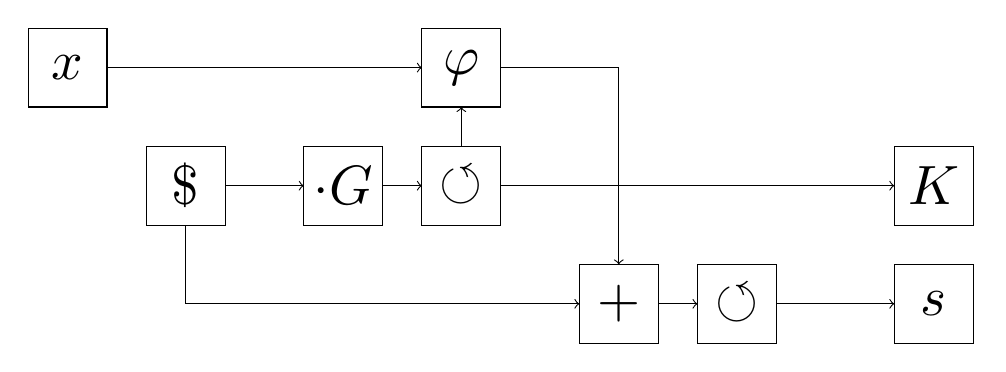
\begin{tikzpicture}[y=-1cm]
    \draw (0,0) rectangle (1,1) node[pos=0.5, scale=2.0] {$x$};
    \draw (1.5,1.5) rectangle (2.5,2.5) node[pos=0.5, scale=2.0] {$\$$};
    \draw (3.5,1.5) rectangle (4.5,2.5) node[pos=0.5, scale=2.0] {$\cdot G$};
    \draw (5.0,1.5) rectangle (6.0,2.5) node[pos=0.5, scale=2.0] {$\circlearrowleft$};
    \draw (5.0,0.0) rectangle (6.0,1) node[pos=0.5, scale=2.0] {$\varphi$};
    \draw (7.0,3.0) rectangle (8.0,4.0) node[pos=0.5, scale=2.0] {$+$};
    \draw (8.5,3.0) rectangle (9.5,4.0) node[pos=0.5, scale=2.0] {$\circlearrowleft$};
    \draw (11,3.0) rectangle (12,4.0) node[pos=0.5, scale=2.0] {$s$};
    \draw (11,1.5) rectangle (12,2.5) node[pos=0.5, scale=2.0] {$K$};
    \draw [->] (1, 0.5) -- (5.0, 0.5);
    \draw [->] (2.5, 2.0) -- (3.5, 2.0);
    \draw [->] (4.5, 2.0) -- (5.0, 2.0);
    \draw [->] (5.5, 1.5) -- (5.5, 1.0);
    \draw [->] (6.0, 2.0) -- (11, 2.0);
    \draw [->] (2.0, 2.5) -- (2.0, 3.5) -- (7.0, 3.5);
    \draw [->] (6.0, 0.5) -- (7.5, 0.5) -- (7.5, 3.0);
    \draw [->] (8.0, 3.5) -- (8.5, 3.5);
    \draw [->] (9.5, 3.5) -- (11, 3.5);
\end{tikzpicture}
\end{afigure}

Figure \ref{fig:schnorr} presents the circuit for Schnorr signatures,
with $\circlearrowleft$ denoting reconstruction nodes,
$\$$ denoting random input nodes, and $\varphi$ denoting
the parameterized homomorphism:
$$
\varphi(K)(x) := H(K, m) \cdot x
$$
Both the $\varphi$ and $+$ nodes have a depth of $2$, and thus so
does the circuit.

Using our semantics for circuits, we get a semi-honest protocol for
threshold Schnorr signatures. The quorum turns their threshold
secret sharing of the secret key $x$ into a linear secret sharing $\shared{x}$.
They then generate a shared nonce $\shared{k}$ by each sampling
$k_i \xleftarrow{R} \Zq$. They calculate a sharing $\shared{K := k \cdot G}$
by each computing $K_i := k_i \cdot G$. They then reveal these $K_i$ to
learn $K$. They can then compute $s_i := \varphi(K)(x_i)$ locally,
creating a sharing $\shared{s}$, whose shares they then reveal,
to learn $s$. They then use $(K, s)$ as their signature.

\subsection{Normalized Form}

While the formal definition of GRCs above is complete, and closely
matches the description of various functionalities, it's not
particularly convenient to design a protocol for.
We can vastly simplify the description of a GRC through the use
of a \emph{normalized form}, which is a much more compact representation
of this circuit.
This normalized form is also directly amenable to an implementation
as an MPC protocol.
This form is derived from a series of simple transformations on
a GRC.

First, note that the random input nodes of the GRC do not depend on
any other node.
Because of this, we can move all of these nodes
to the start of the circuit.
This has the semantics of generating
all the randomness in the circuit at the start of the execution.

Second, instead of having several input nodes $x^1, \ldots, x^m$,
all elements of $\Zq$, we
instead have a single input \emph{vector} $\bx \in \Zq^m$.
This vector can also be considered as a single element of the product
group, with addition defined pointwise, as in Section \ref{sec:background}.
In fact, we can also include random elements as part of the input.
Honest parties will generate this part of the input
randomly for each execution.
We treat this issue in more detail in Section \ref{sec:mpc_prot}.

Third, we can make each $\varphi$ node depend on the entire
input vector $\bx$.
In practice, this dependency can be sparse: $\varphi$
may only make use of a small number of elements in the input.
Nonetheless, $\varphi$ is still a homomorphism with respect
to the entire input.
This is because a projection $\pi : \Zq^m \to \Zq^l$, which selects
a subset of elements from an input vector, is a group homomorphism.
Any homomorphism using only a subset of elements can be composed with $\pi$
to make a homomorphism over the entire vector.

Fourth, we can coalesce the homomorphisms together, creating one
homomorphism for each ``layer'' of the circuit.
We do this by first organizing the $\varphi$ nodes into layers,
based on their depth.
Each node with the same depth goes into the same layer.
We then combine all of the homomorphisms in this layer into
a single homomorphism $\varphi$.
We can do this because the duplication map $a \mapsto (a, a)$
and the projection map $(a, \_) \mapsto a$ are both homomorphisms.
We can sort all of the homomorphisms in a layer topologically, and then compose
them sequentially, duplicating the input and projecting as necessary.

Fifth, we can remove reconstruction nodes.
Because each layer only has a single homomorphism, we can consider
the output of this homomorphism to necessarily be reconstructed.
We then make each homomorphism parameterized by all of the reconstructed
outputs from each previous layer.

Finally, we can remove output nodes.
By considering the output of every layer to be part of the output,
we include all of the output nodes connected to reconstruction nodes.
For the other outputs, they can be locally computed using the reconstructed
outputs along with the shares of the input vector, so it's not necessary
to include them in the circuit.

Combining all of these transformations gives us the formal description of normalized form
GRCs in Figure \ref{fig:grc}.

\begin{afigure}{fig:grc}{GRCs in normalized form}
A group reconstruction circuit (GRC) in normalized form consists of:
\begin{itemize}
    \item An input length $m$, and a depth $d$.
    \item Groups $\mathbb{B}_1, \ldots, \mathbb{B}_d$.
    \item Homomorphisms $\varphi_1, \ldots, \varphi_d$. Each $\varphi_i$
    is a homomorphism $\Zq^m \to \mathbb{B}_i$, and is parameterized
    by values $\bV_1, \ldots, \bV_{i - 1}$ with $\bV_i \in \mathbb{B}_i$.
\end{itemize}
\end{afigure}

We can also give circuits in this form semantics
as a semi-honest MPC protocol.
The parties have a linear secret sharing $\shared{\bx}$ of
the input vector, some entries of which having been generated randomly
for this execution.
Then, for each layer $r \in [d]$, the parties locally
compute ${}\bV_r^i := \varphi_r(\bV_1, \ldots, \bV_{r - 1})(\bx^i)$,
and then reveal these shares, allowing each party to compute
$\bV_r := \sum_i \bV_r^i$.
The values $\bV_1, \ldots, \bV_d$ make up the output of the protocol.

In Section \ref{sec:applications}, we provide examples of GRCs
in normalized form for several functionalities, including Schnorr
signatures.

\section{MPC Protocol for GRCs}
\label{sec:mpc_prot}

In this section, we describe an MPC protocol for computing
a GRC on linearly shared inputs, with associated commitments.
We analyze the security of this protocol, proving that it
is secure against an arbitrary number of malicious parties,
and under concurrent composition, in the UC framework.

For inputs, one natural kind of commitment are Pedersen commitments.
In many protocols, however, it's more natural to use plain commitments,
where a scalar $x$ is committed to with the value $x \cdot G$.
This matches most threshold Schnorr schemes,
in which the secret $x$ is split into shares $x_i$, with the shares
of the public key $X_i := x_i \cdot G$ being known for all parties.
While we could subsume these commitments as a case of Pedersen commitments,
with a blinding factor set to $0$, explicitly considering these
plain commitments yields a more efficient protocol.

We thus split our input vector into three sections: $\bx$, $\by$, and $\bk$.
Each of this is linearly split into shares.
We have shares $\bx^1, \ldots, \bx^n$ for each party, such that $\bx = \sum_i \bx^i$,
and similarly for $\by$ and $\bk$.
The shares of $\bx$ have plain commitments $\bX^i = \bx_i \cdot G$
for each party.
The shares of $\by$ have Pedersen commitments $\bY^i = \by_i \cdot G + \balpha^i \cdot H$,
with $\balpha^i$ a vector of blinding factors held by each party.
Finally, $\bk$ is intended to be randomly generated for each execution
of the protocol.
Honest parties will generate their share $\bk^i$ by sampling a random
vector.
As long as at least one participant in the protocol is honest,
then $\bk := \sum_i \bk^i$ will also be random.

\subsection{Ideal Functionality}
\label{sec:idealfunc}
In this section, we describe an ideal functionality for our protocol,
as Functionality \ref{fun:mpc}.
This functionality is parameterized by the circuit $\Phi$,
as well as the input commitments $\bX^i$ and $\bY^i$, for each party
$i \in [n]$.
The functionality also uses a common reference string $(G, H) \in \mathbb{G}^2$,
for Pedersen commitments.

\begin{afunctionality}{fun:mpc}{GRC functionality $\mathcal{F}(\texttt{GRC}, \Phi, \textbf{X}^i, \textbf{Y}^i)$}
A functionality $\mathcal{F}$ for parties $P_1, \ldots, P_n$.\\
\\
After receiving
$(\texttt{input}, \texttt{sid}, \textbf{x}^i, \textbf{y}^i, \boldsymbol{\alpha}^i, \textbf{k}^i)$ from every party $P_i$:\\
$\mathcal{F}$ checks, for every $i \in [n]$, that:
$$
\begin{aligned}
    \textbf{X}^i &\stackrel{?}{=} \textbf{x}^i \cdot G\\
    \textbf{Y}^i &\stackrel{?}{=} \textbf{y}^i \cdot G + \boldsymbol{\alpha}^i \cdot H\\
\end{aligned}
$$
$\mathcal{F}$ computes, for each round $r \in [d]$:
$$
\begin{aligned}
    \textbf{V}^i_{r} &:= \varphi_{r}(\textbf{V}_{1}, \ldots, \textbf{V}_{r - 1})(
        \textbf{x}^i, \textbf{y}^i, \textbf{k}^i
    )\\
    \textbf{V}_r &:= \sum_j \textbf{V}^i_r
\end{aligned}
$$\\
$\mathcal{F}$ sends $(\texttt{output}, \texttt{sid}, \textbf{V}^1_1, \ldots, \textbf{V}^n_d)$ to every party $P_i$.
\end{afunctionality}

This functionality checks that the inputs each party provides match
the public commitments, and then computes the output of the circuit
in a straightforward manner.
One slight difference is that instead of simply learning $\bV_r$ for
every round $r$, each party learns $\bV^i_r$ for every party $i$.
Naturally, we have $\bV_r = \sum_i \bV^i_r$, so this information
can be derived by each party.
The reason we allow the parties to also learn the individual shares
is that our protocol will also reveal this
information, so we need to model the leakage in our functionality as well.
Furthermore, this matches the semantics of GRCs,
where parties learn the individual shares of the group element they're
reconstructing.
For practical functionalities like Schnorr signatures or threshold encryption,
learning these intermediate values is not a concern either.

\subsection{Protocol}

In this section, we provide a protocol implementing Functionality
\ref{fun:mpc}.

The basic idea is that for each round $r$, the parties locally
compute $\bV^i_r := \varphi_r(\bx^i, \by^i, \bk^i)$, and then
send these values to the other parties, along with a proof that
the value was computed correctly, and that the inputs used correspond
to the public commitments.

For the random input $\bk^i$, we need to guarantee that the same
input vector is used throughout the protocol.
We do this by creating a Pedersen commitment $\bK^i$ to the random value,
and having an initial round where each party broadcasts this commitment
to the other parties.
To prevent a party from sending different commitments, we
use Functionality \ref{fun:broadcast} to guarantee that the same
commitment is sent to all parties.

We can easily prove that each step was computed correctly, and with the right
inputs, by using the following homomorphism:
$$
\psi_r(\textbf{x}, \textbf{y}, \boldsymbol{\alpha}, \textbf{k}, \boldsymbol{\beta})
:= (\varphi_r(\bx, \by, \bk),\ \bx \cdot G,\ \by \cdot G + \balpha \cdot H,\
\bk \cdot G + \bbeta \cdot H) 
$$
This homomorphism uses the same inputs to compute $\varphi_r$
and reconstruct all of the commitments.
We then combine this with the $\varphi$-proofs seen in Section \ref{sec:maurer} to
create an efficient sigma protocol verifying
that a value $\bV^i_r$ was computed using $\varphi_r$ on the correct
inputs.
We then use Functionality \ref{fun:zk} to turn these sigma protocols
into non-interactive proof of knowledge functionalities.

Protocol \ref{prot:mpc} describes all of this more formally.
Like the ideal functionality, the protocol is parameterized by
the circuit $\Phi$, the public commitments $\bX^i, \bY^i$, and makes
use of a common reference string $(G, H) \in \mathbb{G}^2$, for Pedersen
commitments.
The protocol takes $d + 1$ rounds, with $d$ the depth of the circuit.
As we mentioned in the previous section, the parties learn
the intermediate values $\bV^i_r$ as a consequence of the protocol's
execution.

\begin{aprotocol}{prot:mpc}{MPC protocol for $\Phi, \textbf{X}^i, \textbf{Y}^i$}

Each party $P_i$ has inputs $\textbf{x}^i$ and $\textbf{y}^i$, committed to
by $\textbf{X}^i$ and $\textbf{Y}^i$.
They also have decommitments $\boldsymbol{\alpha}^i$ for $\textbf{Y}^i$.
Each party $P_i$ also has a vector $\textbf{k}^i$, which honest parties will
have generated randomly.\\
\\
\textbf{Round 0}\\
Each party $P_i$ generates a random vector $\boldsymbol{\beta}^i$, and creates
a commitment to $\textbf{k}^i$ with:
$$
\textbf{K}^i := \bk^i \cdot G + \bbeta^i \cdot H
$$
$P_i$ sends $(\texttt{broadcast-in}, \texttt{sid}, \textbf{K}^i)$ to
the broadcast functionality $\mathcal{C}$.\\
$P_i$ waits to receive $(\texttt{broadcast-out}, \texttt{sid}, \textbf{K}^j)$
for each other party $j$.\\
\\
\textbf{Round $r$}\\
Each party $P_i$ computes $\bV^i_r := \varphi_r(\bV_1, \ldots, \bV_{r - 1})(\bx^i, \by^i, \bk^i)$.\\
Each party $P_i$ sends $(\texttt{prove}, \texttt{sid}, (\bx^i, \by^i, \balpha^i, \bk^i, \bbeta^i))$
to $\mathcal{F}(\texttt{ZK}, \psi_r)$, receiving $\pi^i_r$ in return.\\
Each party $P_i$ sends $(\bV^i_r, \pi^i_r)$ to every other party.\\
\\
After receiving $(\bV^j_r, \pi^j_r)$  from all other parties, $P_i$ checks,
for each $j$, that the proof is valid, by sending $(\texttt{verify}, (\bV^j_r, \bX^j, \bY^j, \bK^j), \pi^j_r)$ to
$\mathcal{F}(\texttt{ZK}, \psi_r)$, and aborting if the functionality returns $0$.\\
Each party $P_i$ then stores each $\bV^j_r$ as part of its output,
and computes $\bV_r := \sum_j \bV^j_r$.
\end{aprotocol}

\subsection{Security Analysis}

In this section, we prove that Protocol \ref{prot:mpc} implements
Functionality \ref{fun:mpc} with UC security, even against an arbitrary
number of malicious parties.
More specifically, we work with the SUC model of security~\cite{canetti_simpler_2015}.
We also work in the hybrid model, using Functionalities
\ref{fun:zk} and \ref{fun:broadcast} for zero-knowledge proofs of knowledge,
and authenticated broadcast, respectively.
We also need a common reference string $(G, H) \in \mathbb{G}^2$, for
Pedersen commitments.
In our proof, the simulator provides this string.

\begin{theorem}
Provided that the discrete logarithm is hard in $\mathbb{G}$, Protocol \ref{prot:mpc} securely implements Functionality \ref{fun:mpc},
in the hybrid model of universally composable security,
given a non-interactive $\varphi$-proof functionality $\mathcal{F}(\text{ZK}, \varphi)$ (for arbitrary $\varphi$),
a broadcast functionality $\mathcal{C}$, as well as a common reference string
${(G, H) \in \mathbb{G}^2}$.
\end{theorem}
\textbf{Proof Idea:}\\
The basic idea is that we use an instance of the discrete logarithm problem
as our common reference string.
This makes any violation of the binding property of Pedersen commitments
yield a solution to this discrete logarithm instance.
Otherwise, we can perfectly simulate an execution of the protocol
using the ideal functionality, without rewinding
the adversary, which lets us conclude that our protocol is UC secure,
using the result in \cite{kushilevitz_information-theoretically_2009}.

One technical detail is that we need inputs from every party
to give to the ideal functionality.
Because of this, our simulator first runs the simulated protocol
until the adversary provides the input for their parties in the first proof.
We can then use these values for the parties the simulator controls
in the ideal functionality.

The output of this functionality gives us all of the values we need
in the rest of the simulation, except for the commitments $\bK^i$
to the random inputs of the honest parties.
For these, we use the fact that Pedersen commitments are perfectly
hiding, and simply generate them at random.

\textbf{Proof:}\\
We prove this by constructing a simulator $\calS$ which uses
the ideal functionality $\mathcal{F}(\texttt{GRC})$ to perfectly
simulate an execution of the hybrid protocol against an adversary
$\mathcal{A}$.

We also work in the common reference string model, where the simulator
$\mathcal{S}$ chooses the generators $G, H$ for the Pedersen commitments.

We use this simulator $\calS$ to construct an adversary against
the discrete logarithm game.

Let $\calM \subseteq \calP$ be the set of malicious parties,
and $\calH \subseteq \calP$ be the set of honest parties. Naturally,
we have $\calH \cup \calM = \calP$ and $\calH \cap \calM = \emptyset$.

As an adversary against the discrete logarithm game,
$\calS$ receives $(G, H)$ as an instance 
of the discrete logarithm problem.

The simulator then proceeds as follows:\\
$\calS$ starts by setting $(G, H)$ as the common reference string.

\textbf{Round 0}:\\
For each $i \in \calH$, $\calS$ samples $\bK^i \xleftarrow{R} \mathbb{G}$.\\
For each $i \in \calM$,
$\calS$ waits to receive $(\texttt{broadcast-in}, \texttt{sid}, \bK^i)$.\\
$\calS$ then sends $(\texttt{broadcast-out}, \texttt{pid}_i, \texttt{sid}, \bK^i)$,
to all parties, for every $i \in \calP$, emulating $\mathcal{C}$.

\textbf{Interim}:\\
$\calS$ waits to receive $(\texttt{prove}, \texttt{sid}, (\bx^i, \by^i, \balpha^i, \bk^i, \bbeta^i))$
for each malicious ${i \in \calM}$,
playing the role of $\mathcal{F}(\texttt{ZK}, \psi_1)$.\\
$\calS$ checks, for each $i$, that:
$$
\begin{aligned}
\bX^i &\stackrel{?}{=} \bx^i \cdot G\\
\bY^i &\stackrel{?}{=} \by^i \cdot G + \balpha^i \cdot H\\
\bK^i &\stackrel{?}{=} \bk^i \cdot G + \bbeta^i \cdot H
\end{aligned}
$$
otherwise, $\calS$ sets $\texttt{bad-values}^i_1 \gets 1$.\\
$\calS$ records the values $\bx^i, \by^i, \balpha^i, \bk^i, \balpha^i$, for $i \in \calM$.\\

Now, in the real execution against $\mathcal{F}(\texttt{GRC})$,
with real honest parties $P_i$, for
each $i \in \calM$, the parties $\calS$ controls, $\calS$ sends
$(\texttt{input}, \texttt{sid}, \bx^i, \by^i, \balpha^i, \bk^i)$ to $\mathcal{F}(\texttt{GRC})$.\\
$\calS$ receives $(\texttt{output}, \texttt{sid}, \bV^1_1, \ldots, \bV^n_d)$ in return,
and records these values.

\textbf{Round $r$}:\\
For each round $r \in [d]$, $\calS$ proceeds as follows:\\
$\calS$ generates a new $\pi^j_r$ for each $j \in \calH$, and sends
$(\bV^j_r, \pi^j_r)$ to every malicious $P_i$, with $i \in \calM$.

Unless $r = 1$, $\calS$ waits to receive 
$(\texttt{prove}, \texttt{sid}, \hat{\bx}^i, \hat{\by}^i, \hat{\balpha}^i, \hat{\bk}^i, \hat{\bbeta}^i)$
from each malicious $P_i$, for $i \in \calM$, playing the role of $\mathcal{F}(\texttt{ZK}, \psi_r)$.\\
$\mathcal{S}$ then checks, for each $i$, that:
$$
\begin{aligned}
\bX^i &\stackrel{?}{=} \hat{\bx}^i \cdot G\\
\bY^i &\stackrel{?}{=} \hat{\by}^i \cdot G + \hat{\balpha}^i \cdot H\\
\bK^i &\stackrel{?}{=} \hat{\bk}^i \cdot G + \hat{\bbeta}^i \cdot H
\end{aligned}
$$
and sets $\texttt{bad-values}^i_r \gets 1$ otherwise.\\
The first check implies that $\hat{\bx}^i = \bx^i$. If it holds that
$\hat{\by}^i \neq \by^i$ or $\hat{\bk}^i \neq \bk^i$, then $\calS$ has
found a value $h$ such that $h \cdot G = H$, as per Lemma \ref{lemma:ped_vec_dlog},
and $\calS$ aborts, returning $h$.

(Including when $r = 1$) $\calS$ generates a new $\pi^i_r$, and returns $(\texttt{proof}, \pi^i_r)$,
playing the role of $\mathcal{F}(\texttt{ZK}, \psi_r)$.

Concurrently, $\calS$ plays the role of $\mathcal{F}(\texttt{ZK}, \psi_r)$,
responding to $(\texttt{verify}, (\hat{\bV}^j_r, \hat{\bX}^j, \hat{\bY}^j, \hat{\bK}^j), \pi)$
queries. $\calS$ checks that there exists some $i \in \mathcal{P}$ such that
$\pi^i_r = \pi$. $\calS$ then returns:
$$
\hat{\bV}^j_r \stackrel{?}{=} \bV^j_r \land
\hat{\bX}^j \stackrel{?}{=} \bX^j \land
\hat{\bY}^j \stackrel{?}{=} \bY^j \land
\hat{\bK}^j \stackrel{?}{=} \bK^j \land
\texttt{bad-values}^i_r \neq 1
$$

$\calS$ then waits to receive $(\hat{\bV}^i, \hat{\pi}^i_r)$ for
every malicious party $P_i$, with ${i \in \mathcal{M}}$.\\
$\calS$ then checks if the query $(\texttt{verify}, (\hat{\bV^i_r}, \bX^i, \bY^i, \bK^i), \hat{\pi}^i_r)$
would yield $1$, according to the logic in the section above.
(If $\hat{\pi}^i_r$ doesn't match anything, the check is considered to fail).
If this check fails, then $\calS$ simulates every honest $P_j$ aborting, with $j \in \calH$,
to abort, as if they'd seen an invalid proof themselves.

This concludes the simulation.

If $\calS$ aborts with a value $h$, then they've successfully
solved an instance of the discrete logarithm problem. Under our
assumption that this problem is hard, this happens with negligible
probability.

We argue that if $\calS$ does not abort in this way, then the simulation
is perfect. For the first round, because pedersen commitments
are perfectly hiding, sampling a random $\bK^i$ has an identical
distribution as an honest party generating a pedersen commitment.
For the rest of the protocol, all of our checks are equivalent
to those made by honest parties. This is because the
$\bV^j_i$ values are necessarily computed correctly, and use
the inputs provided by the parties the adversary $\mathcal{A}$ controls.

Because our simulator $\calS$ is perfect, and doesn't
rewind the adversary $\mathcal{A}$, we conclude,
using~\cite{kushilevitz_information-theoretically_2009},
that our protocol
satisfies universally composable security, in the hybrid model.

$\qed$

\subsubsection{Identifiable Abort}

We note that our protocol can be considered to have identifiable
aborts, provided that the implementation of the broadcast functionality
also has this property.
After round $0$, if a party causes an abort by providing an invalid
proof, then that abort can be detected, since there will be
a signed message containing this invalid proof, which can be used
as evidence of cheating.

\subsection{Practical Considerations}

In this section we describe a few additional details which might
be useful for concrete implementations of the protocol.

\subsubsection{Sparse Proofs}

For simplicity, we have each homomorphism $\varphi_i$ in the circuit
take the entire input vector $\bx$.
These homomorphisms may be \emph{sparse}, in the sense
that they only use a few of the elements in the input vector.
It should be noted that in this case, the $\varphi$-proofs can
be done as if only these select elements existed, which gives
a smaller and faster proof.

\subsubsection{Removing Random Commitments}

Some functionalities may not use any random input $\bk$.
In this case, the first round can be omitted, since there's
no need to commit to an empty vector.
This actually improves the complexity of threshold encryption,
as we'll see in Section \ref{sec:threshold_enc}.

\subsubsection{Parallel Echos}

In the description of our protocol, we use one round for broadcasting
the commitments to the random inputs, using our broadcast functionality.
If we naively replace this functionality with the
echo-broadcast in Protocol \ref{prot:echo},
we increase the round complexity, since that protocol requires 2 rounds.
However, the second round of the echo-broadcast protocol is only
needed to check the consistency of the broadcasted input; the parties
already know the input after the first round.
Because of this, we can run this second round \emph{in parallel}
with the rest of the protocol, and thus incur no additional
cost to round complexity. 

\subsubsection{Parallel $\texttt{sid}$}

While there are different ways of instantiating
the non-interactive proofs of knowledge Functionality \ref{fun:zk}, some of them
heavily rely on the use of a unique session identifier $\texttt{sid}$.
Because this particular identifier isn't needed in the first round,
we can run a session identifier agreement protocol,
such as~\cite{barak_protocol_2004}, in parallel with the first round.
This improves the round complexity of the concrete protocol as
compared to sequential composition.

\subsection{Complexity}

The round complexity of our protocol is near-optimal, with
only one additional round to provide commitments to random inputs,
which can be omitted if the circuit doesn't use them.

We also argue that the concrete complexity of our protocol
compares favorably with more specialized protocols.
As noted before, the basic approach of locally computing
the homomorphisms matches the basic strategy of specialized protocols.
The overhead in our case comes from the additional $\varphi$-proofs
we need to include, as well as computing additional commitments
for the random inputs.
Thankfully, these proofs are quite efficient.
The cost of each proof is dominated by that of computing
$\varphi$ along with 1 or 2 scalar multiplications per input, to prove that
the right inputs were used.
While more expensive than specialized protocols,
this is nonetheless a manageable amount of overhead for
a generic protocol.

\section{Applications}
\label{sec:applications}

In this section, we describe several applications of our protocol,
by providing concrete GRCs
for various functionalities.
We also compare the complexity of our generic protocol,
instantiated on these circuits, with specialized
protocols computing the same functionality.

\subsection{Distributed Key Generation}
\label{sec:dkg}

Distributed Key Generation (DKG) can be formulated in terms of group
reconstruction circuits.
This allows us to create a DKG protocol where the parties
generate a common public key $X$, and where each party has
a share $x_i$ of the private key, such that $\sum_i x_i \cdot G = x \cdot G = X$.

We can formulate this as a GRC by having $x$ be considered a
random input to the protocol. 
Our circuit then consists of the single homomorphism:
$$
\varphi(x) := x \cdot G
$$

Concretely, the protocol works by having each party
generate a random share $x_i$, and broadcasting a Pedersen commitment
$K_i$.
The parties then send $x_i \cdot G$, along with a proof that
this value matches the commitment $K_i$ sent previously.
The parties implicitly learn $x_i$ through this process,
even though this output isn't explicitly considered in the description
of the circuit.


\subsection{Threshold Schnorr Signatures}
\label{sec:schnorr}

We've described the Schnorr signature functionality as a GRC before,
but not yet in normalized form. In this form, our input consists
of the private signature key $x$, as well as the nonce $k$.
We then have two homomorphisms:
$$
\begin{aligned}
    \varphi_1(x, k) &:= k \cdot G\\
    \varphi_2(K)(x, k) &:= k + H(K, m) \cdot x
\end{aligned}
$$

We can then instantiate our protocol with this circuit to get a
threshold signature scheme, assuming that some other distributed
key generation scheme is used.
Given a threshold sharing of the private key $x$,
we assume that a quorum of parties can generate a linear sharing
of $x$ as $x_1 + \ldots + x_n$, along with public key shares $X_i := x_i \cdot G$.
This assumption matches the standard polynomial schemes used
for threshold secret sharing, where Lagrange interpolation is used
to derive linear shares.
Using these linear shares, the parties then run our protocol
to compute a signature.

The round complexity of this signing protocol matches
that 3 round scheme of Lindell \cite{lindell_simple_2022}.
The only additional security assumption we make is the hardness
of the discrete logarithm in $\mathbb{G}$, which makes our protocol
relatively conservative, as Lindell's scheme purports to be.
The concrete complexity of our protocol is a bit higher, because of
the extra proofs we need to compute, and our use of Pedersen commitments.

Our protocol compares disfavorably against 2 round signing protocols
such as FROST \cite{komlo_frost_2020}, or MuSig2 \cite{nick_musig2_2021},
which also have better concrete complexity.

\subsection{Threshold Encryption}
\label{sec:threshold_enc}

We can create a threshold encryption scheme, by adapting
ElGamal encryption \cite{elgamal_public_1985}.
In this scheme, the ciphertext contains a group element $R \in \mathbb{G}$,
and the value $x \cdot R$ needs to be computed, using the private key
$x \in \Zq$. 

This can naturally be described as a GRC, with a single input $x$,
and a homomorphism:
$$
\varphi_1(x) := x \cdot R
$$

Using the same key generation assumptions as for Schnorr signatures,
we get a threshold encryption scheme.
A quorum decrypts a message by deriving linear shares $x = x_1 + \ldots + x_n$
of the private key, along with commitments $X_i := x_i \cdot G$,
and then using our protocol to learn the value $x \cdot R$,
which allows each party to decrypt the message.
Our protocol also guarantees that the output matches the public key $X$.

We can skip the initial round, since no random input is needed,
making our protocol only take a single round, which is optimal.

\subsection{Polynomial Openings}

The polynomial commitment scheme of Kate et al.~\cite{kate_constant-size_2010}
provides an efficient scheme for committing to a polynomial
$f \in \mathbb{F}_q[X]$, as well as for computing evaluation witnesses.
These witness are short proofs that a value $f(z)$ corresponds
to the evaluation of the committed polynomial $f$ at the point $z$.

We can capture both the commitment and evaluation procedures
using the formalism of GRCs.
This gives us a protocol for computing a commitment to a
threshold-shared polynomial, as well as for evaluating that polynomial,
and creating a witness for that evaluation.

We recapitulate only the necessary details of these schemes,
referring the reader to the full paper by Kate et al. for the remaining
details.
The commitment scheme assumes the existence of a trusted
setup $G_0, \ldots, G_t \in \mathbb{G}$, satisfying a special relationship,
and allowing commitments for polynomials of degree $t$.

A commitment to a polynomial is computed as:
$$
\text{Com}(f) := \sum_i f_i \cdot G_i
$$
with $f_0, \ldots, f_t$ denoting the coefficients of that polynomial.

An evaluation witness for $f$ at the point $z$ is computed by defining
the polynomial:
$$
\psi_f(X) := \frac{f(X) - f(z)}{(X - z)}
$$
and then computing the witness as $\text{Com}(\psi_f)$.

If we interpret polynomials $f \in \mathbb{F}_q[X]$ of degree $t$
as vectors $\textbf{f} \in \Zq^{(t + 1)}$, 
then we realize that both of these functionalities are already
GRCs.
This is because $\text{Com}$ and $f \mapsto \psi_f$ are both
homomorphisms with respect to the vector $\textbf{f}$.

For $\text{Com}$ this is evident.
On the other hand, for calculating $\psi_f$, it's not immediately
clear that this is homomorphic.
First, note that polynomial evaluation is homomorphic:
$f(z) + g(z) = (f + g)(z)$.
Thus, $f(X) - f(z)$ is also homomorphic with respect of $f$.
Finally, note that division by a polynomial is also homomorphic.
If $f(X) = q_f(X) p(x)$, and $g(X) = q_g(X) p(X)$, then $(f + g)(X) = (q_f + q_g)(X) p(X)$.

Thus, both functionalities consist of a single homomorphism
on the input vector, and are thus implementable as GRCs.

\section{Limitations and Further Work}

In this work, we presented the formalism
of group reconstruction circuits (GRC)s, as well as a simple
protocol for computing them on secret shared inputs in the
malicious setting.
We expect future work to expand upon this formalism,
and improve upon the protocol we've provided.
In this section, we suggest several potential improvements
to our formalism and the protocol we've described.

\subsection{Intermediate Values}

Functionality \ref{fun:mpc}, which our protocol implements,
has the side effect of leaking the intermediate values
$\bV^1_r, \ldots, \bV^n_r$ at each round,
rather than just their sum $\bV_r := \sum_i \bV^i_r$.
For functionalities like Schnorr signatures, this doesn't
reveal information about the secrets,
but this may not be the case in general.
A potential improvement would be to design a protocol
such that only the sum $\bV_r$ is revealed in each round.

\subsection{Aggregating Commitments}

Our current protocol commits to vectors of values by using
independent commitments.
An alternative would be to commit to the entire vector
with a single commitment.
We would do this by using independent generators $G_1, \ldots, G_m$,
and then defining commitments as the following sum:
$$
\text{Com}(\by, \alpha) := r\cdot H + \sum_i \by_i \cdot G_i
$$
Using these commitments have the advantage of a smaller communication cost.
The computation cost would be slightly improved as well, since we have a single
blinding factor $\alpha$, rather than an entire vector.

Directly applying this change would be disadvantageous for sparse homomorphisms.
Proofs would no longer be faster for such homomorphisms.
This is because
the commitment now relies on the entire input vector, and so
our proofs would need to use the entire input,
even if the homomorphism for that round only used a small portion of that vector. 

Further work might find a way to have the advantages of single
element commitments, while also mitigating the overhead
for sparse homomorphisms.

\subsection{Aggregating Proofs}

Currently, our protocol requires verifying
$(n - 1) \cdot d$ proofs: one for each layer, and each other party.
A natural improvement would be to try aggregating these
proofs, to reduce the cost of verifying them.
This could be done by combining the proofs of different parties
in a given round, or even combining proofs across different rounds.
While $\varphi$-proofs have the advantage of being
simple and efficient, they're not directly aggregatable, nor
are they concise.
We conjecture that improvements on these fronts might come from
exploring other proof techniques.

\subsection{Exploiting Circuit Structure}

One advantage of the GRC formalism is that our protocol
can be used to implement a large number of functionalities.
A disadvantage is that the protocol is less efficient compared
to protocols tailored to a specific functionality.
Further work might be able to close this gap by exploiting
specific patterns in circuits, while nonetheless
remaining general.

If we look at the DKG protocol of Section \ref{sec:dkg},
we include a proof that we know $x_i$ and $\beta$ such that
$x_i \cdot G = X_i$ and $x_i \cdot G + \beta \cdot H = K_i$.
We do this via a $\varphi$-proof, but in this specific case,
we could more efficiently prove this by simply revealing $\beta$.
There's no need to hide $x_i \cdot G$ in this case, since the
other parties learn this anyways.
This pattern could be exploited more generally as well.

As another example, if we look at the Schnorr signature
protocol we end up with in Section \ref{sec:schnorr},
we include a proof that the partial signature $s_i := k_i + H(K, m) \cdot x_i$
was computed correctly.
This proof is in fact redundant, because it suffices to verify
the final signature computed by the protocol is valid.
This is another repeatable pattern, wherein many functionalities
are \emph{self-verifying}, to a certain extent,
in the sense that the output already has some means of validation.
Further work could try and more precisely quantify what
this property means, and to what extent it can replace the use
of proofs inside the protocol.

\subsection{Threshold Interpretations}

One limitation of our current semantics for GRCs is that we require
the inputs to have a \emph{linear} secret sharing.
It might be interesting to explore an alternative interpretation
in which we work directly with inputs using a threshold secret sharing,
throughout the entire protocol.

For example, in our DKG protocol, we produce linear shares
of the public key.
Most applications would rather have a threshold secret sharing
instead.
Instead of interpreting the random nodes in our GRC
by having each party generate their own linear share, we could
instead use a verifiable secret sharing (VSS) protocol,
such as \cite{feldman_practical_1987}, and create a threshold
secret sharing of this random value.
Applying this to the DKG circuit, we would get a protocol
directly usable for generating keys for threshold encryption
or signing.

This alternative interpretation could also be useful
for signing or encryption as well, in order to create a more robust protocol.
If we take Schnorr signatures as an example,
our current protocol takes the approach of first having the quorum
of signers derive a linear secret sharing of the secret,
and then having the entire quorum interact throughout the remainder
of the protocol.
The disadvantage of this approach is that we can't tolerate
any failures from the signers after the start of the protocol,
even if more than a threshold remain.
In contrast, the protocol of Stinson et al.~\cite{stinson_provably_2001},
can continue as long as at least a threshold of signers
remains, tolerating failures.
It does this by using threshold secret sharings for every value,
which ensures that the parties will be able to reconstruct
the final signature, provided at least a threshold remains
by the end of the execution.
Using a threshold interpretation of GRCs would bring this
kind of robustness to a variety of different functionalities.

\section{Conclusion}

In this work, we generalized various functionalities, including
signatures, encryption, and polynomial commitments,
under the novel formalism of \emph{group reconstruction circuits} (GRC)s.

We then constructed an efficient MPC protocol to compute these circuits
on secret shared inputs, and proved it to be UC secure against
malicious adversaries.

This construction immediately yields UC secure protocols for threshold Schnorr
signatures, ElGamal encryption, and polynomial commitments.

While we've given a handful of examples of how GRCs can be used
in this work, we hope that they might prove useful for other functionalities,
given their generality.
Hopefully, further work can improve on the simple protocol we've
constructed in this work, further closing the gap between
functionality-specific and generic protocols.

\bibliographystyle{splncs04}
\bibliography{bib}
\end{document}
